%===============================================================================
% LaTeX sjabloon voor de graduaatsproef Programmeren aan HOGENT
% Meer info op https://github.com/HoGentPRG/latex-hogent-report
%===============================================================================

\documentclass[dutch,dit,thesis]{hogentreport}

% TODO:
% - If necessary, replace the option `dit`' with your own department!
%   Valid entries are dbo, dbt, dgz, dit, dlo, dog, dsa, soa
% - If you write your thesis in English (remark: only possible after getting
%   explicit approval!), remove the option "dutch," or replace with "english".

\usepackage{lipsum} % For blind text, can be removed after adding actual content

%% Pictures to include in the text can be put in the graphics/ folder
\graphicspath{{../graphics/}}

%% For source code highlighting, requires pygments to be installed
%% Compile with the -shell-escape flag!
%% \usepackage[chapter]{minted}
%% If you compile with the make_thesis.{bat,sh} script, use the following
%% import instead:
\usepackage[chapter,outputdir=../output]{minted}
\usemintedstyle{solarized-light}

%% Formatting for minted environments.
\setminted{%
    autogobble,
    frame=lines,
    breaklines,
    linenos,
    tabsize=4
}

%% Ensure the list of listings is in the table of contents
\renewcommand\listoflistingscaption{%
    \IfLanguageName{english}{Lijst van codefragmenten}{List of listings}
}
\renewcommand\listingscaption{%
    \IfLanguageName{english}{Codefragment}{Listing}
}
\renewcommand*\listoflistings{%
    \cleardoublepage\phantomsection\addcontentsline{toc}{chapter}{\listoflistingscaption}%
    \listof{listing}{\listoflistingscaption}%
}

% Other packages not already included can be imported here

%%---------- Document metadata -------------------------------------------------
% TODO: Replace this with your own information
\author{Sheylene Bos}
\supervisor{Dhr. Luc Vervoort}
% \cosupervisor{Mevr. S. Beeckman}
\title[C++ verkennen met game dev]%
    {C++ and SFML}
\academicyear{\advance\year by -1 \the\year--\advance\year by 1 \the\year}
\examperiod{1}
\degreesought{\IfLanguageName{english}{Graduaat in het Programmeren}{Associate of applied computer science}}
\partialthesis{false} %% To display 'in partial fulfilment'
%\institution{Internshipcompany BVBA.}

%% Add global exceptions to the hyphenation here
\hyphenation{back-slash}

%% The bibliography (style and settings are  found in hogentthesis.cls)
 \addbibresource{gradproef.bib}            %% Bibliography file
% \addbibresource{../voorstel/voorstel.bib} %% Bibliography research proposal
% \defbibheading{bibempty}{}

%% Prevent empty pages for right-handed chapter starts in twoside mode
\renewcommand{\cleardoublepage}{\clearpage}

\renewcommand{\arraystretch}{1.2}

%% Content starts here.
\begin{document}

%---------- Front matter -------------------------------------------------------

\frontmatter

\hypersetup{pageanchor=false} %% Disable page numbering references
%% Render a Dutch outer title page if the main language is English
\IfLanguageName{english}{%
    %% If necessary, information can be changed here
    \degreesought{Graduaat in het Programmeren}%
    \begin{otherlanguage}{english}%
       \maketitle%
    \end{otherlanguage}%
}{}

%% Generates title page content
\maketitle
\hypersetup{pageanchor=true}
%%=============================================================================
%% Samenvatting
%%=============================================================================

% TODO: De "abstract" of samenvatting is een kernachtige (~ 1 blz. voor een
% thesis) synthese van het document.
%
% Een goede abstract biedt een kernachtig antwoord op volgende vragen:
%
% 1. Waarover gaat de graduaatsproef?
% 2. Waarom heb je er over geschreven?
% 3. Hoe heb je het onderzoek uitgevoerd?
% 4. Wat waren de resultaten? Wat blijkt uit je onderzoek?
% 5. Wat betekenen je resultaten? Wat is de relevantie voor het werkveld?
%
% Daarom bestaat een abstract uit volgende componenten:
%
% - inleiding + kaderen thema
% - probleemstelling
% - (centrale) onderzoeksvraag
% - onderzoeksdoelstelling
% - methodologie
% - resultaten (beperk tot de belangrijkste, relevant voor de onderzoeksvraag)
% - conclusies, aanbevelingen, beperkingen
%
% LET OP! Een samenvatting is GEEN voorwoord!

%%---------- Nederlandse samenvatting -----------------------------------------
%
% TODO: Als je je graduaatsproef in het Engels schrijft, moet je eerst een
% Nederlandse samenvatting invoegen. Haal daarvoor onderstaande code uit
% commentaar.
% Wie zijn/haar graduaatsproef in het Nederlands schrijft, kan dit negeren, de inhoud
% wordt niet in het document ingevoegd.

\IfLanguageName{dutch}{
\selectlanguage{dutch}
\chapter*{Samenvatting}

Op het einde van onze opleiding hebben we de opdracht gekregen om een nieuwe programmeertaal te leren en een project te maken in deze taal. 
We konden kiezen om ofwel bij ons stagebedrijf een project te doen, ofwel een project te doen met een zelfgekozen onderwerp.
\\
\\
Ik heb ervoor gekozen om zelfstandig in C++ een game te maken met Unreal Engine 5. 
Dit project is een grote uitdaging geweest, omdat ik nog nooit eerder met C++ of Unreal Engine 5 had gewerkt.
Sommige concepten van de taal waren mij bekend omdat ik al eerder met C\# had gewerkt, maar de taal zelf was nieuw voor mij.
In het begin was ik begonnen met onderzoek naar de taal en de engine, tegelijkertijd onderzocht ik of er mogelijkheden waren 
de game efficienter te maken met behulp van design patterns.

Later schakelde ik over naar SFML, omdat Unreal Engine 5 niet goed werkte en ik meer wilde focussen op de taal zelf.
}

%%---------- Samenvatting -----------------------------------------------------
% De samenvatting in de hoofdtaal van het document

\chapter*{\IfLanguageName{dutch}{Summary}{Summary}}

At the end of our studies, we were given the assignment to learn a new programming language and create a project using this language.
We could choose either to do a project at our internship company or to work on a self-chosen topic.
\\
\\
I chose to independently create a game in C++ using Unreal Engine 5.
This project was a major challenge, as I had never worked with C++ or Unreal Engine 5 before.
Some concepts of the language were familiar to me because I had previously worked with C\#, but the language itself was new to me.
In the beginning, I started by researching the language and the engine, while also investigating whether there were possibilities to make the game more efficient using design patterns.

%---------- Inhoud, lijst figuren, ... -----------------------------------------

\tableofcontents

% In a list of figures, the complete caption will be included. To prevent this,
% ALWAYS add a short description in the caption!
%
%  \caption[short description]{elaborate description}
%
% If you do, only the short description will be used in the list of figures

% \listoffigures

% If you included tables and/or source code listings, uncomment the appropriate
% lines.
% \listoftables

% \listoflistings

% Als je een lijst van afkortingen of termen wil toevoegen, dan hoort die
% hier thuis. Gebruik bijvoorbeeld de ``glossaries'' package.
% https://www.overleaf.com/learn/latex/Glossaries

%---------- Kern ---------------------------------------------------------------

\mainmatter{}

% De eerste hoofdstukken van een graduaatsproef zijn meestal een inleiding op
% het onderwerp, literatuurstudie en verantwoording methodologie.
% Aarzel niet om een meer beschrijvende titel aan deze hoofdstukken te geven of
% om bijvoorbeeld de inleiding en/of stand van zaken over meerdere hoofdstukken
% te verspreiden!

%%=============================================================================
%% Inleiding
% De inleiding moet de lezer net genoeg informatie verschaffen om het onderwerp te begrijpen en in te zien waarom de onderzoeksvraag de moeite waard is om te onderzoeken. In de inleiding ga je literatuurverwijzingen beperken, zodat de tekst vlot leesbaar blijft. Je kan de inleiding verder onderverdelen in secties als dit de tekst verduidelijkt. Zaken die aan bod kunnen komen in de inleiding~\autocite{Pollefliet2011}:
% Uit je probleemstelling moet duidelijk zijn dat je onderzoek een meerwaarde heeft voor een concrete doelgroep. De doelgroep moet goed gedefinieerd en afgelijnd zijn. Doelgroepen als ``bedrijven,'' ``KMO's'', systeembeheerders, enz.~zijn nog te vaag. Als je een lijstje kan maken van de personen/organisaties die een meerwaarde zullen vinden in deze bachelorproef (dit is eigenlijk je steekproefkader), dan is dat een indicatie dat de doelgroep goed gedefinieerd is. Dit kan een enkel bedrijf zijn of zelfs één persoon (je co-promotor/opdrachtgever).
% Wees zo concreet mogelijk bij het formuleren van je onderzoeksvraag. Een onderzoeksvraag is trouwens iets waar nog niemand op dit moment een antwoord heeft (voor zover je kan nagaan). Het opzoeken van bestaande informatie (bv. ``welke tools bestaan er voor deze toepassing?'') is dus geen onderzoeksvraag. Je kan de onderzoeksvraag verder specifiëren in deelvragen. Bv.~als je onderzoek gaat over performantiemetingen, dan 
% Wat is het beoogde resultaat van je graduaatsproef? Wat zijn de criteria voor succes? Beschrijf die zo concreet mogelijk. Gaat het bv.\ om een proof-of-concept, een prototype, een verslag met aanbevelingen, een vergelijkende studie, enz.

% Het is gebruikelijk aan het einde van de inleiding een overzicht te
% geven van de opbouw van de rest van de tekst. Deze sectie bevat al een aanzet
% die je kan aanvullen/aanpassen in functie van je eigen tekst.


% TODO: Vul hier aan voor je eigen hoofstukken, één of twee zinnen per hoofdstuk

%%=============================================================================

\chapter{\IfLanguageName{dutch}{Inleiding}{Introduction}}%
\label{ch:inleiding}


C++ is een taal dat ontstond in de jaren '80 en is een uitbreiding van de programmeertaal C.
Zelfs als het al 40 jaar oud is, is het nog steeds een van de meest populaire programmeertalen ter wereld.
Het wordt vaak gebruikt voor systeemsoftware, game-ontwikkeling en toepassingen die hoge prestaties vereisen. De geschiedenis van informatica 
boeit me, vooral de evolutie van programmeertalen. Omdat C++ zo lang bestaat, zijn er veel verschillende versies van de taal. 
De concepten en technieken die in C++ worden gebruikt, bestaan er voor een reden.
C++ biedt een combinatie van lage-niveau geheugenbeheer en hoge-niveau abstractie, waardoor het een veelzijdige taal is voor verschillende soorten 
softwareontwikkeling.


\section{\IfLanguageName{dutch}{Wat is c++?}{Wat is c++?}}%
\label{sec:Wat is c++?}


In de jaren 70 werden er veel programmeertalen ontwikkeld, hieronder C, Pascal en Fortran voorbeelden hiervan.
Deze talen hadden veel limieten, zoals het gebrek aan objectgeoriënteerd programmeren en het gebrek aan lage-niveau geheugenbeheer.
Bjarne Stroustrup, een Deense computerwetenschapper, begon in 1979 met het ontwikkelen van C++ als een uitbreiding van de programmeertaal C.
C++ is een programmeertaal die de kracht van C combineert met de mogelijkheden van objectgeoriënteerd programmeren.


Het is een veelzijdige taal die vandaag de dag gebruikt wordt voor verschillende soorten softwareontwikkeling, zoals systeemsoftware, game-ontwikkeling en toepassingen die hoge prestaties vereisen.
De ontwikkelaar van de taal haalde inspiratie uit verschillende programmeertalen, zoals Simula, C, Algol 68 en andere talen om C++ te ontwikkelen.
Simula was de pionier op het gebied van objectgeoriënteerd programmeren en introduceerde concepten zoals klassen en objecten.
Het was een taal die kind was van de taal Algol 60, die op zijn beurt weer een invloed had op de ontwikkeling van C.
Later werd Angol 60 herzien en werd het Angol 68.
Terwijl Angol 68 een taal was die invloed heeft gehad op het structureren van code, deze taal introduceerde het gebruik van code blokken.


C++ krijgt elke 3 jaar een nieuwe versie, maar meestal gebruiken programmeers de oudere versies van de compiler.
Er bestaaan ook meerdere verschillende IDEs die C++ ondersteunen, 
zoals Microsoft Visual Studio, Code::Blocks en CLion.  

\section{\IfLanguageName{dutch}{Wat is SFML?}{What is SFML?}}%
\label{sec:Wat is SFML?}

SFML (Simple and Fast Multimedia Library) is een cross-platform software development library ontworpen om een eenvoudige API te bieden voor het programmeren van multimedia applicaties. 
Het is geschreven in C++ en biedt bindingen voor andere talen zoals C, .NET, Python, Java, en meer.
SFML biedt modules voor 2D graphics, audio, windowing, en netwerkfunctionaliteit. 
Het wordt vaak gebruikt voor het ontwikkelen van 2D games en andere interactieve grafische applicaties.


\section{\IfLanguageName{dutch}{Toelichting van mijn keuze}{Research question}}%
\label{sec:Toelichting van mijn keuze}

Ik heb ervoor gekozen om C++ te leren voor mijn graduaatsproef omdat er veel concepten zijn die mij interessant lijken. 
Deze concepten kunnen mij ook helpen bij het schrijven van software in andere programmeertalen. Memory management kennen helpt bij het begrijpen 
van hoe variabelen in het geheugen worden opgeslagen en hoe ze worden beheerd. Pointers en references zijn essentiële concepten 
die ervoor zorgen dat er geen onnogidige kopieën van gegevens worden gemaakt, wat de prestaties van een programma kan verbeteren. 
Dynamische allocatie kan bijleren hoe gegeugen kan gefragmenteerd worden en hoe je dit kan voorkomen. 
Wanneer ik over C++ lees, zie ik vaak dat het een heel krachtige taal is, maar dat het ook complex kan zijn. 
Tijdens mijn graduaatsproef wil ik zelf ervaren hoe het voelt om met C++ te werken en de kracht van de taal te ontdekken. 
Een andere motivatie is dat ik mijn studie wil verder zetten naar een bacheloropleiding. Een mogelijke taal die ik daar kan leren is C++, 

Daarnaast leek SFML interessant voor mij. Het zorgt ervoor dat ik de taal kan leren kennen in
omgeving die creatief is en waar ik mijn eigen ideeën kan uitwerken. 
Er bestaat ook een mogelijkheid om tijdens de zomer verder te werken aan het project, wat mij de kans geeft om meer bij te leren.

\section{\IfLanguageName{dutch}{Onderzoeksdoelstelling}{Research objective}}%
\label{sec:onderzoeksdoelstelling}
Het doel van deze graduaatsproef is C++ te leren kennen en de verschillen tussen 
C++ en C\#, dat wij tijdens deze opleiding hebben geleerd, te ontdekken. 

\section{\IfLanguageName{dutch}{Opzet van deze graduaatsproef}{Structure of this associate thesis}}%
\label{sec:opzet-graduaatsproef}

De rest van deze graduaatsproef is als volgt opgebouwd:

In Hoofdstuk~\ref{ch:stand-van-zaken} wordt een overzicht gegeven van de stand van zaken binnen het onderzoeksdomein, op basis van een literatuurstudie.

In Hoofdstuk~\ref{ch:methodologie} wordt de methodologie toegelicht en worden de gebruikte onderzoekstechnieken besproken om een antwoord te kunnen formuleren op de onderzoeksvragen.


In Hoofdstuk~\ref{ch:conclusie}, tenslotte, wordt de conclusie gegeven en een antwoord geformuleerd op de onderzoeksvragen. Daarbij wordt ook een aanzet gegeven voor toekomstig onderzoek binnen dit domein.
\chapter{\IfLanguageName{dutch}{Stand van zaken}{State of the art}}%
\label{ch:stand-van-zaken}

% Tip: Begin elk hoofdstuk met een paragraaf inleiding die beschrijft hoe
% dit hoofdstuk past binnen het geheel van de graduaatsproef. Geef in het
% bijzonder aan wat de link is met het vorige en volgende hoofdstuk.

% Pas na deze inleidende paragraaf komt de eerste sectiehoofding.

% In C++, declarations usually go 
% into header files, typically with extension .h, while definitions usually go into source files, typically 
% with extension .cpp.

C++ maakt gebruik van verschillende filetypes zoals header files (\texttt{.h} of \texttt{.hpp}) en source files (\texttt{.cpp}).
Header files bevatten de declaraties van functies, klassen, variabelen en interfaces. De source files zijn de definities van de headerfiles en bevatten de implementatie van de functies en methodes.
Source files worden gecompileerd naar object files (\texttt{.o} of \texttt{.obj}), die vervolgens worden gelinkt om een uitvoerbaar bestand te maken.
Waarom dit gedaan wordt, is om de code beter te organiseren en herbruikbaarheid te bevorderen. Door de scheiding van declaraties en implementaties kunnen verschillende delen van een programma onafhankelijk worden ontwikkeld en gecompileerd.
\\

Helemaal in het begin van een C++-programma staat de \texttt{\#include}-directive, die aangeeft welke header files moeten worden opgenomen.
Dit wordt anders gedaan dan in C\#, waar de \texttt{using}-directive wordt gebruikt om namespaces te importeren.
De implementatie van zelfgeschreven klassen gebruiken de headerfile "" terwijl de standaardbibliotheek van C++ gebruik maakt van <> voor andere packages.
Voor Unreal Engine is het echter anders, de standaardbibliotheek wordt er niet gebruikt.
Dit komt door de geschiedenis van de taal. In de jaren 90 werden de standaardbibliotheken geintruduceert.
Rond dezelfde tijd werd ook de Unreal Engine ontwikkeld. 
De standaardbibliotheek maakte toen gebuik van nieuwe features van C++. 
Het was een probleem want sommige features werden niet goed getest en de kans ontstond dat de code niet werkte zoals verwacht.
Daarnaast waren de bibliotheken slecht geimplementeerd, hadden ze veel bugs en waren ze heel controversieel.
Als gevolg kozen ze ervoor om de standaardbibliotheek niet te gebruiken en in plaats daarvan hun eigen bibliotheek te ontwikkelen.

\\

De data types in C++ zijn niet zo uitgebreid als in C\#, maar de basis types zoals \texttt{int}, \texttt{float}, \texttt{double} en \texttt{char} zijn aanwezig.
C++ heeft ook een \texttt{string}-type, maar dit is niet zo uitgebreid als in C\#. In C++ worden strings vaak behandeld als arrays van tekens, wat kan leiden tot meer complexiteit bij het werken met strings.
Er moet van de standaardbibliotheek de string header file worden opgenomen om met strings te werken.
Dictionaries en lijsten zijn in C++ niet ingebouwd in de taal zoals ze zijn in C\#. In plaats daarvan worden ze vaak geïmplementeerd met behulp van arrays of de STL (Standard Template Library).
\\

Wat er ook anders is in C++ is dat een klasse kan overerven van meerdere klassen, wat niet mogelijk is in C\#. Dit lijkt mij bijzonder nuttig. Zolang de 2 klassen geen namen hebben die hetzelfde zijn, kan er geen verwarring ontstaan.


Unreal Engine maakt gebruik van een andere manier van classen en objecten dan C++. In Unreal Engine worden klassen gedefinieerd met behulp van de \texttt{UCLASS}-macro, die aangeeft dat de klasse een Unreal Engine-klasse is.
Tijdens mijn onderzoek waren er enkele problemen die ervoor zorgden dat ik niet verder kon met het project.
Verschillende keren moest ik de hele project opnieuw opbouwen omdat hij de classen niet kon terugvinden.
Dan was er ook het probleem dat Visual Studio Enterprise soms bestanden verstopte van mij, waardoor ik dacht dat ze helemaal verdwenen waren.
Het probleem was dat de klassen moesten worden toegevoegd via de Unreal Engine Editor, anders werden ze niet herkend door de engine.
Het is hoogst waarschijnlijk dat dit op een andere manier kan worden opgelost, maar ik heb er niet veel tijd in gestoken om het uit te zoeken.
\\

Het project moest ik meerdere keren opnieuw herstarten omdat ik iets nieuws vond en het moest toepassen.
De huidige structuur werkte niet mee met het idee, dus er waren stukken van code die opnieuw schreef.
\\
Andere momenten waren er problemen met het crashen van ofwel Unreal Engine of Visual Studio.
De programma's laden heel traag, en daarbij was het niet zeldzaam dat er af en toe een crash gebeurde.
\\

Voor mijn project had ik ervoor gekozen om design patterns te gebruiken.
Daarvoor werd er eerst grondig onderzoek gedaan naar welke design patterns nuttig zouden zijn .
Documentatie werd geraadpleegd tijdens mijn literatuurstudie hierover in C++.
Zo wordt er bijvoorbeeld gebruik gemaakt van de Simple Factory Pattern, voor items zoals wapens en voedsel.
Dan is er ook de Observer Pattern, die ervoor zorgt dat de UI altijd up-to-date is met de laatste informatie van de speler.
De Factory Method Pattern wordt gebruikt om verschillende soorten vijanden te maken, afhankelijk van de situatie.

Naast de reeds genoemde patterns, zijn er nog andere die zeer nuttig kunnen zijn in Unreal Engine:

De \textbf{Component Pattern} is handig om gameobjecten flexibel samen te stellen uit verschillende herbruikbare componenten, zoals gezondheid, beweging, of inventaris. Unreal Engine gebruikt dit principe zelf in zijn Actor Component systeem.

De \textbf{Command Pattern} kan worden ingezet om acties van de speler of AI te encapsuleren als objecten. Dit is nuttig voor het implementeren van undo/redo functionaliteit, het opslaan en later uitvoeren van commando's (bv. voor replays of AI-planning), of het ontkoppelen van de actie-uitvoerder van de actie-initiator.

De \textbf{Strategy Pattern} maakt het mogelijk om algoritmes of gedrag uit te wisselen tijdens runtime, bijvoorbeeld voor verschillende bewegingspatronen van vijanden of AI.

De \textbf{Decorator Pattern} kan gebruikt worden om dynamisch extra functionaliteit toe te voegen aan objecten, zoals power-ups of tijdelijke effecten bij een speler of vijand.

De \textbf{Service Locator Pattern} biedt een alternatieve manier om globale services (zoals audio, input, of logging) toegankelijk te maken zonder overal afhankelijkheden te injecteren.

Deze patronen helpen om de code schaalbaar, onderhoudbaar en uitbreidbaar te houden, zeker bij grotere projecten in Unreal Engine.
\\

Tegelijkertijd probeerde ik de taal en de engine te leren kennen.
Ik heb ervoor gezorgd dat ik niet blind code overneem van anderen, maar dat de code ook klopte en dat ik het begreep.
Meestal schreef ik zelf de code omdat de tutorials niet altijd duidelijk waren en ze meestal blueprints gebruiken.
Als ik wel blueprints gebruikte dan was het voor de visuele representatie van de code.
Er werd ervoor gezorgd dat de meeste delen van de code in C++ werden geschreven.
\\

Daarnaast is er ook een inventory systeem gemaakt, dat ervoor zorgt dat de speler items kan verzamelen en gebruiken.





% \textcite{Knuth1998} schreef een van de standaardwerken over sorteer- en zoekalgoritmen. Experten zijn het erover eens dat cloud computing een interessante opportuniteit vormen, zowel voor gebruikers als voor dienstverleners op vlak van informatietechnologie~\autocite{Creeger2009}.

% Let er ook op: het \texttt{cite}-commando voor de punt, dus binnen de zin. Je verwijst meteen naar een bron in de eerste zin die erop gebaseerd is, dus niet pas op het einde van een paragraaf.

% \begin{figure}
%   \centering
%   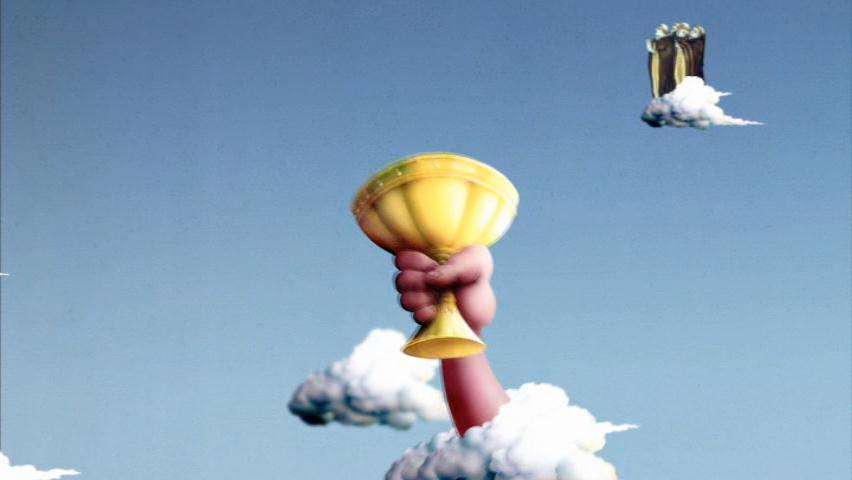
\includegraphics[width=0.8\textwidth]{grail.jpg}
%   \caption[Voorbeeld figuur.]{\label{fig:grail}Voorbeeld van invoegen van een figuur. Zorg altijd voor een uitgebreid bijschrift dat de figuur volledig beschrijft zonder in de tekst te moeten gaan zoeken. Vergeet ook je bronvermelding niet!}
% \end{figure}

% \begin{listing}
%   \begin{minted}{python}
%     import pandas as pd
%     import seaborn as sns

%     penguins = sns.load_dataset('penguins')
%     sns.relplot(data=penguins, x="flipper_length_mm", y="bill_length_mm", hue="species")
%   \end{minted}
%   \caption[Voorbeeld codefragment]{Voorbeeld van het invoegen van een codefragment.}
% \end{listing}

% \lipsum[7-20]

% \begin{table}
%   \centering
%   \begin{tabular}{lcr}
%     \toprule
%     \textbf{Kolom 1} & \textbf{Kolom 2} & \textbf{Kolom 3} \\
%     $\alpha$         & $\beta$          & $\gamma$         \\
%     \midrule
%     A                & 10.230           & a                \\
%     B                & 45.678           & b                \\
%     C                & 99.987           & c                \\
%     \bottomrule
%   \end{tabular}
%   \caption[Voorbeeld tabel]{\label{tab:example}Voorbeeld van een tabel.}
% \end{table}


%%=============================================================================
%% Methodologie
%%=============================================================================

\chapter{\IfLanguageName{dutch}{Methodologie}{Methodology}}%
\label{ch:methodologie}

%% TODO: In dit hoofstuk geef je een korte toelichting over hoe je te werk bent
%% gegaan. Verdeel je onderzoek in grote fasen, en licht in elke fase toe wat
%% de doelstelling was, welke deliverables daar uit gekomen zijn, en welke
%% onderzoeksmethoden je daarbij toegepast hebt. Verantwoord waarom je
%% op deze manier te werk gegaan bent.
%% 
%% Voorbeelden van zulke fasen zijn: literatuurstudie, opstellen van een
%% requirements-analyse, opstellen long-list (bij vergelijkende studie),
%% selectie van geschikte tools (bij vergelijkende studie, "short-list"),
%% opzetten testopstelling/PoC, uitvoeren testen en verzamelen
%% van resultaten, analyse van resultaten, ...
%%
%% !!!!! LET OP !!!!!
%%
%% Het is uitdrukkelijk NIET de bedoeling dat je het grootste deel van de corpus
%% van je graduaatsproef in dit hoofstuk verwerkt! Dit hoofdstuk is eerder een
%% kort overzicht van je plan van aanpak.
%%
%% Maak voor elke fase (behalve het literatuuronderzoek) een NIEUW HOOFDSTUK aan
%% en geef het een gepaste titel.

De graduaatsproef begon met een literatuurstudie over C++ in het algemeen. Er werd opgezocht hoe de verschillende concepten van de taal werken.
Verschillende bronnen werden geraadpleegd, zoals boeken, online tutorials en documentatie van de taal zelf. 
Sommige bronnen waren meer gericht op beginners, terwijl andere meer diepgaand waren en zich richtten op gevorderde gebruikers.
Op het einde van de studie werden de fundamenten gelegd voor het project zodat ze toegepast konden worden.
\\

De volgende stap was experimenteren met de taal zelf in Microsoft Visual Studio.
Een paar kleine projecten werden gemaakt om de basisconcepten van de taal te begrijpen, zoals variabelen, loops, functies en classes.
Deze projecten hielpen met de syntax en mechanismen van de taal te begrijpen. 
Tijdens de finale versie met Unreal Engine 5 zou er dan teruggevallen kunnen worden op deze kennis.
\\

Tenslotte er dan begonnen met het finale project in Unreal Engine 5.
De opzetting van het project werd gedaan en Unreal Engine werd bestudeerd.
Een Proof of Concept werd gemaakt als een finale deel van de graduaatsproef.



% Voeg hier je eigen hoofdstukken toe die de ``corpus'' van je graduaatsproef
% vormen. De structuur en titels hangen af van je eigen onderzoek. Je kan bv.
% elke fase in je onderzoek in een apart hoofdstuk bespreken.

%\input{...}
%\input{...}
%...

%%=============================================================================
%% Conclusie
%%=============================================================================

\chapter{Conclusie}%
\label{ch:conclusie}

% TODO: Trek een duidelijke conclusie, in de vorm van een antwoord op de
% onderzoeksvra(a)g(en). Wat was jouw bijdrage aan het onderzoeksdomein en
% hoe biedt dit meerwaarde aan het vakgebied/doelgroep? 
% Reflecteer kritisch over het resultaat. In Engelse teksten wordt deze sectie
% ``Discussion'' genoemd. Had je deze uitkomst verwacht? Zijn er zaken die nog
% niet duidelijk zijn?
% Heeft het onderzoek geleid tot nieuwe vragen die uitnodigen tot verder 
%onderzoek?

Het beginnnen aan mijn project was niet makkelijk. 
Als ik iets van ervaring had, dan zou ik meteen gestart kunnen zijn met het maken van de game.
Uitdagingen worden vaak verwelkomt door mij en ik had wel plezier tijdens het studeren.
De onderzoek naar de geschiedenis boeide mij enorm. 
Ik heb geleerd hoe je moet doorzetten terwijl je vast zit.
Twijfelen gebeurde veel, maar ik heb ervoor gezorgd dat ik niet opgaf.
\\

Ik kan toegeven dat ik liever een project had gemaakt zonder Unreal Engine, met enkel C++.
Het visuele gedeelte van Unreal Engine was zenuwverwekkend door de tijdsgebrek.
Door de stage was het moeilijk om tijd te vinden om aan het project te werken.
SFML is een bibliotheek dat ik heel snel gekozen had, omdat het een eenvoudige API biedt voor het programmeren van multimedia applicaties.
Ik wou meer focussen op de taal zelf en niet op de engine. Lieft had ik vanaf het begin zo gewerkt, maar ik heb er veel van geleerd.
Omdat ik zo weinig ervaring had met Unreal Engine, leek het mogelijk te zijn om veel code te schrijven hiervoor.
Dat zou wel misschien mogelijk geweest zijn, maar door de obstakels die ik tegenkwam, was het moeilijk om verder te gaan.
Daarom was het een opluchting dat ik snel kon overstappen naar SFML.

De taal zelf leren was een gedeelte waarvan ik genoot en in de toekomst wil ik er zeker mee verder gaan.






%---------- Bijlagen -----------------------------------------------------------

% \appendix

% \chapter{Onderzoeksvoorstel}

% Het onderwerp van deze graduaatsproef is gebaseerd op een onderzoeksvoorstel dat vooraf werd beoordeeld door de promotor. Dat voorstel is opgenomen in deze bijlage.

%% TODO: 
%\section*{Samenvatting}

% Kopieer en plak hier de samenvatting (abstract) van je onderzoeksvoorstel.

% Verwijzing naar het bestand met de inhoud van het onderzoeksvoorstel
% %---------- Inleiding ---------------------------------------------------------

% TODO: Is dit voorstel gebaseerd op een paper van Research Methods die je
% vorig jaar hebt ingediend? Heb je daarbij eventueel samengewerkt met een
% andere student?
% Zo ja, haal dan de tekst hieronder uit commentaar en pas aan.

%\paragraph{Opmerking}

% Dit voorstel is gebaseerd op het onderzoeksvoorstel dat werd geschreven in het
% kader van het vak Research Methods dat ik (vorig/dit) academiejaar heb
% uitgewerkt (met medesturent VOORNAAM NAAM als mede-auteur).
% 

\section{Inleiding}%
\label{sec:inleiding}

Waarover zal je graduaatsproef gaan? Introduceer het thema en zorg dat volgende zaken zeker duidelijk aanwezig zijn:

\begin{itemize}
  \item kaderen thema
  \item de doelgroep
  \item de probleemstelling en (centrale) onderzoeksvraag
  \item de onderzoeksdoelstelling
\end{itemize}

Denk er aan: een typische graduaatsproef is \textit{toegepast onderzoek}, wat betekent dat je start vanuit een concrete probleemsituatie in bedrijfscontext, een \textbf{casus}. Het is belangrijk om je onderwerp goed af te bakenen: je gaat voor die \textit{ene specifieke probleemsituatie} op zoek naar een goede oplossing, op basis van de huidige kennis in het vakgebied.

De doelgroep moet ook concreet en duidelijk zijn, dus geen algemene of vaag gedefinieerde groepen zoals \emph{bedrijven}, \emph{developers}, \emph{Vlamingen}, enz. Je richt je in elk geval op it-professionals, een bachelorproef is geen populariserende tekst. Eén specifiek bedrijf (die te maken hebben met een concrete probleemsituatie) is dus beter dan \emph{bedrijven} in het algemeen.

Formuleer duidelijk de onderzoeksvraag! De begeleiders lezen nog steeds te veel voorstellen waarin we geen onderzoeksvraag terugvinden.

Schrijf ook iets over de doelstelling. Wat zie je als het concrete eindresultaat van je onderzoek, naast de uitgeschreven scriptie? Is het een proof-of-concept, een rapport met aanbevelingen, \ldots Met welk eindresultaat kan je je bachelorproef als een succes beschouwen?

%---------- Stand van zaken ---------------------------------------------------

\section{Literatuurstudie}%
\label{sec:literatuurstudie}

Hier beschrijf je de \emph{state-of-the-art} rondom je gekozen onderzoeksdomein, d.w.z.\ een inleidende, doorlopende tekst over het onderzoeksdomein van je graduaatsproef. Je steunt daarbij heel sterk op de professionele \emph{vakliteratuur}, en niet zozeer op populariserende teksten voor een breed publiek. Wat is de huidige stand van zaken in dit domein, en wat zijn nog eventuele open vragen (die misschien de aanleiding waren tot je onderzoeksvraag!)?

Je mag de titel van deze sectie ook aanpassen (literatuurstudie, stand van zaken, enz.). Zijn er al gelijkaardige onderzoeken gevoerd? Wat concluderen ze? Wat is het verschil met jouw onderzoek?

Verwijs bij elke introductie van een term of bewering over het domein naar de vakliteratuur, bijvoorbeeld~\autocite{Hykes2013}! Denk zeker goed na welke werken je refereert en waarom.

Draag zorg voor correcte literatuurverwijzingen! Een bronvermelding hoort thuis \emph{binnen} de zin waar je je op die bron baseert, dus niet er buiten! Maak meteen een verwijzing als je gebruik maakt van een bron. Doe dit dus \emph{niet} aan het einde van een lange paragraaf. Baseer nooit teveel aansluitende tekst op eenzelfde bron.

Als je informatie over bronnen verzamelt in JabRef, zorg er dan voor dat alle nodige info aanwezig is om de bron terug te vinden (zoals uitvoerig besproken in de lessen Research Methods).

% Voor literatuurverwijzingen zijn er twee belangrijke commando's:
% \autocite{KEY} => (Auteur, jaartal) Gebruik dit als de naam van de auteur
%   geen onderdeel is van de zin.
% \textcite{KEY} => Auteur (jaartal)  Gebruik dit als de auteursnaam wel een
%   functie heeft in de zin (bv. ``Uit onderzoek door Doll & Hill (1954) bleek
%   ...'')

Je mag deze sectie nog verder onderverdelen in subsecties als dit de structuur van de tekst kan verduidelijken.

%---------- Methodologie ------------------------------------------------------
\section{Methodologie}%
\label{sec:methodologie}

Hier beschrijf je hoe je van plan bent het onderzoek te voeren. Welke onderzoekstechniek ga je toepassen om elk van je onderzoeksvragen te beantwoorden? Gebruik je hiervoor literatuurstudie, interviews met belanghebbenden (bv.~voor requirements-analyse), experimenten, simulaties, vergelijkende studie, risico-analyse, PoC, \ldots?

Valt je onderwerp onder één van de typische soorten graduaatsproeven die besproken zijn in de lessen Research Methods (bv.\ vergelijkende studie of risico-analyse)? Zorg er dan ook voor dat we duidelijk de verschillende stappen terug vinden die we verwachten in dit soort onderzoek!

Vermijd onderzoekstechnieken die geen objectieve, meetbare resultaten kunnen opleveren. Enquêtes, bijvoorbeeld, zijn voor een graduaatsproef informatica meestal \textbf{niet geschikt}. De antwoorden zijn eerder meningen dan feiten en in de praktijk blijkt het ook bijzonder moeilijk om voldoende respondenten te vinden. Studenten die een enquête willen voeren, hebben meestal ook geen goede definitie van de populatie, waardoor ook niet kan aangetoond worden dat eventuele resultaten representatief zijn.

Uit dit onderdeel moet duidelijk naar voor komen dat je graduaatsproef ook technisch voldoen\-de diepgang zal bevatten. Het zou niet kloppen als een graduaatsproef informatica ook door bv.\ een student marketing zou kunnen uitgevoerd worden.

Je beschrijft ook al welke tools (hardware, software, diensten, \ldots) je denkt hiervoor te gebruiken of te ontwikkelen.

Probeer ook een tijdschatting te maken. Hoe lang zal je met elke fase van je onderzoek bezig zijn en wat zijn de concrete \emph{deliverables} in elke fase?

%---------- Verwachte resultaten ----------------------------------------------
\section{Verwacht resultaat, conclusie}%
\label{sec:verwachte_resultaten}

Hier beschrijf je welke resultaten je verwacht. Als je metingen en simulaties uitvoert, kan je hier al mock-ups maken van de grafieken samen met de verwachte conclusies. Benoem zeker al je assen en de onderdelen van de grafiek die je gaat gebruiken. Dit zorgt ervoor dat je concreet weet welk soort data je moet verzamelen en hoe je die moet meten.

Wat heeft de doelgroep van je onderzoek aan het resultaat? Op welke manier zorgt jouw graduaatsproef voor een meerwaarde?

Hier beschrijf je wat je verwacht uit je onderzoek, met de motivatie waarom. Het is \textbf{niet} erg indien uit je onderzoek andere resultaten en conclusies vloeien dan dat je hier beschrijft: het is dan juist interessant om te onderzoeken waarom jouw hypothesen niet overeenkomen met de resultaten.



%%---------- Andere bijlagen --------------------------------------------------
% TODO: Voeg hier eventuele andere bijlagen toe. Bv. als je deze BP voor de
% tweede keer indient, een overzicht van de verbeteringen t.o.v. het origineel.
%\input{...}

%%---------- Backmatter, referentielijst ---------------------------------------

\backmatter{}

\setlength\bibitemsep{15pt} %% Add Some space between the bibliograpy entries
\nocite{*}
\printbibliography[heading=bibintoc]

\end{document}
